\documentclass[twoside]{book}

% Packages required by doxygen
\usepackage{fixltx2e}
\usepackage{calc}
\usepackage{doxygen}
\usepackage{graphicx}
\usepackage[utf8]{inputenc}
\usepackage{makeidx}
\usepackage{multicol}
\usepackage{multirow}
\PassOptionsToPackage{warn}{textcomp}
\usepackage{textcomp}
\usepackage[nointegrals]{wasysym}
\usepackage[table]{xcolor}

% Font selection
\usepackage[T1]{fontenc}
\usepackage{mathptmx}
\usepackage[scaled=.90]{helvet}
\usepackage{courier}
\usepackage{amssymb}
\usepackage{sectsty}
\renewcommand{\familydefault}{\sfdefault}
\allsectionsfont{%
  \fontseries{bc}\selectfont%
  \color{darkgray}%
}
\renewcommand{\DoxyLabelFont}{%
  \fontseries{bc}\selectfont%
  \color{darkgray}%
}
\newcommand{\+}{\discretionary{\mbox{\scriptsize$\hookleftarrow$}}{}{}}

% Page & text layout
\usepackage{geometry}
\geometry{%
  a4paper,%
  top=2.5cm,%
  bottom=2.5cm,%
  left=2.5cm,%
  right=2.5cm%
}
\tolerance=750
\hfuzz=15pt
\hbadness=750
\setlength{\emergencystretch}{15pt}
\setlength{\parindent}{0cm}
\setlength{\parskip}{0.2cm}
\makeatletter
\renewcommand{\paragraph}{%
  \@startsection{paragraph}{4}{0ex}{-1.0ex}{1.0ex}{%
    \normalfont\normalsize\bfseries\SS@parafont%
  }%
}
\renewcommand{\subparagraph}{%
  \@startsection{subparagraph}{5}{0ex}{-1.0ex}{1.0ex}{%
    \normalfont\normalsize\bfseries\SS@subparafont%
  }%
}
\makeatother

% Headers & footers
\usepackage{fancyhdr}
\pagestyle{fancyplain}
\fancyhead[LE]{\fancyplain{}{\bfseries\thepage}}
\fancyhead[CE]{\fancyplain{}{}}
\fancyhead[RE]{\fancyplain{}{\bfseries\leftmark}}
\fancyhead[LO]{\fancyplain{}{\bfseries\rightmark}}
\fancyhead[CO]{\fancyplain{}{}}
\fancyhead[RO]{\fancyplain{}{\bfseries\thepage}}
\fancyfoot[LE]{\fancyplain{}{}}
\fancyfoot[CE]{\fancyplain{}{}}
\fancyfoot[RE]{\fancyplain{}{\bfseries\scriptsize Generated on Sun Feb 21 2016 17\+:24\+:04 for My Project by Doxygen }}
\fancyfoot[LO]{\fancyplain{}{\bfseries\scriptsize Generated on Sun Feb 21 2016 17\+:24\+:04 for My Project by Doxygen }}
\fancyfoot[CO]{\fancyplain{}{}}
\fancyfoot[RO]{\fancyplain{}{}}
\renewcommand{\footrulewidth}{0.4pt}
\renewcommand{\chaptermark}[1]{%
  \markboth{#1}{}%
}
\renewcommand{\sectionmark}[1]{%
  \markright{\thesection\ #1}%
}

% Indices & bibliography
\usepackage{natbib}
\usepackage[titles]{tocloft}
\setcounter{tocdepth}{3}
\setcounter{secnumdepth}{5}
\makeindex

% Hyperlinks (required, but should be loaded last)
\usepackage{ifpdf}
\ifpdf
  \usepackage[pdftex,pagebackref=true]{hyperref}
\else
  \usepackage[ps2pdf,pagebackref=true]{hyperref}
\fi
\hypersetup{%
  colorlinks=true,%
  linkcolor=blue,%
  citecolor=blue,%
  unicode%
}

% Custom commands
\newcommand{\clearemptydoublepage}{%
  \newpage{\pagestyle{empty}\cleardoublepage}%
}


%===== C O N T E N T S =====

\begin{document}

% Titlepage & ToC
\hypersetup{pageanchor=false,
             bookmarks=true,
             bookmarksnumbered=true,
             pdfencoding=unicode
            }
\pagenumbering{roman}
\begin{titlepage}
\vspace*{7cm}
\begin{center}%
{\Large My Project }\\
\vspace*{1cm}
{\large Generated by Doxygen 1.8.7}\\
\vspace*{0.5cm}
{\small Sun Feb 21 2016 17:24:04}\\
\end{center}
\end{titlepage}
\clearemptydoublepage
\tableofcontents
\clearemptydoublepage
\pagenumbering{arabic}
\hypersetup{pageanchor=true}

%--- Begin generated contents ---
\chapter{File Index}
\section{File List}
Here is a list of all documented files with brief descriptions\+:\begin{DoxyCompactList}
\item\contentsline{section}{\hyperlink{ej4a_8c}{ej4a.\+c} \\*El ejercicio 4a de la Practica 1 S\+O\+P\+E\+R }{\pageref{ej4a_8c}}{}
\item\contentsline{section}{\hyperlink{ej4b_8c}{ej4b.\+c} \\*El ejercicio 4b de la Practica 1 S\+O\+P\+E\+R }{\pageref{ej4b_8c}}{}
\item\contentsline{section}{\hyperlink{ej5a_8c}{ej5a.\+c} \\*El ejercicio 5a de la Practica 1 S\+O\+P\+E\+R }{\pageref{ej5a_8c}}{}
\item\contentsline{section}{\hyperlink{ej5b_8c}{ej5b.\+c} \\*El ejercicio 5b de la Practica 1 S\+O\+P\+E\+R }{\pageref{ej5b_8c}}{}
\item\contentsline{section}{\hyperlink{ej8a_8c}{ej8a.\+c} \\*El ejercicio 8a de la Practica 1 S\+O\+P\+E\+R }{\pageref{ej8a_8c}}{}
\item\contentsline{section}{\hyperlink{ej8b_8c}{ej8b.\+c} \\*El ejercicio 8b de la Practica 1 S\+O\+P\+E\+R }{\pageref{ej8b_8c}}{}
\item\contentsline{section}{\hyperlink{ejercicio6_8c}{ejercicio6.\+c} \\*El ejercicio 6 de la Practica 1 S\+O\+P\+E\+R }{\pageref{ejercicio6_8c}}{}
\item\contentsline{section}{\hyperlink{ejercicio9_8c}{ejercicio9.\+c} \\*El ejercicio 9 de la Practica 1 S\+O\+P\+E\+R }{\pageref{ejercicio9_8c}}{}
\end{DoxyCompactList}

\chapter{File Documentation}
\hypertarget{ej4a_8c}{\section{ej4a.\+c File Reference}
\label{ej4a_8c}\index{ej4a.\+c@{ej4a.\+c}}
}


El ejercicio 4a de la Practica 1 S\+O\+P\+E\+R.  


{\ttfamily \#include $<$stdio.\+h$>$}\\*
{\ttfamily \#include $<$stdlib.\+h$>$}\\*
{\ttfamily \#include $<$unistd.\+h$>$}\\*
Include dependency graph for ej4a.\+c\+:
\nopagebreak
\begin{figure}[H]
\begin{center}
\leavevmode
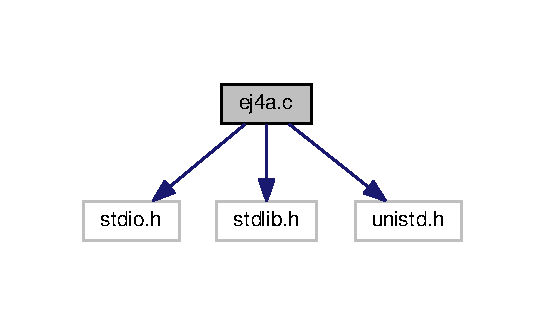
\includegraphics[width=261pt]{ej4a_8c__incl}
\end{center}
\end{figure}
\subsection*{Macros}
\begin{DoxyCompactItemize}
\item 
\hypertarget{ej4a_8c_acee2369f62e4a096d243dec3cd7d0b00}{\#define {\bfseries N\+U\+M\+\_\+\+P\+R\+O\+C}~3}\label{ej4a_8c_acee2369f62e4a096d243dec3cd7d0b00}

\end{DoxyCompactItemize}
\subsection*{Functions}
\begin{DoxyCompactItemize}
\item 
int \hyperlink{ej4a_8c_a840291bc02cba5474a4cb46a9b9566fe}{main} (void)
\begin{DoxyCompactList}\small\item\em Crea procesos Crea 8 procesos y muestras sus P\+I\+D. \end{DoxyCompactList}\end{DoxyCompactItemize}


\subsection{Detailed Description}
El ejercicio 4a de la Practica 1 S\+O\+P\+E\+R. 

\begin{DoxyAuthor}{Author}
Oscar Garcia de Lara Parreño 

Santiago Gomez Aguirre 
\end{DoxyAuthor}
\begin{DoxyVersion}{Version}
1.\+0 
\end{DoxyVersion}
\begin{DoxyDate}{Date}
18-\/02-\/2016 
\end{DoxyDate}


\subsection{Function Documentation}
\hypertarget{ej4a_8c_a840291bc02cba5474a4cb46a9b9566fe}{\index{ej4a.\+c@{ej4a.\+c}!main@{main}}
\index{main@{main}!ej4a.\+c@{ej4a.\+c}}
\subsubsection[{main}]{\setlength{\rightskip}{0pt plus 5cm}int main (
\begin{DoxyParamCaption}
\item[{void}]{}
\end{DoxyParamCaption}
)}}\label{ej4a_8c_a840291bc02cba5474a4cb46a9b9566fe}


Crea procesos Crea 8 procesos y muestras sus P\+I\+D. 

\begin{DoxyReturn}{Returns}
E\+X\+I\+T\+\_\+\+F\+A\+I\+L\+U\+R\+E en caso de error, E\+X\+I\+T\+\_\+\+S\+U\+C\+C\+E\+S\+S si funciona 
\end{DoxyReturn}

\hypertarget{ej4b_8c}{\section{ej4b.\+c File Reference}
\label{ej4b_8c}\index{ej4b.\+c@{ej4b.\+c}}
}


El ejercicio 4b de la Practica 1 S\+O\+P\+E\+R.  


{\ttfamily \#include $<$stdio.\+h$>$}\\*
{\ttfamily \#include $<$stdlib.\+h$>$}\\*
{\ttfamily \#include $<$unistd.\+h$>$}\\*
{\ttfamily \#include $<$sys/wait.\+h$>$}\\*
{\ttfamily \#include $<$sys/types.\+h$>$}\\*
Include dependency graph for ej4b.\+c\+:
\nopagebreak
\begin{figure}[H]
\begin{center}
\leavevmode
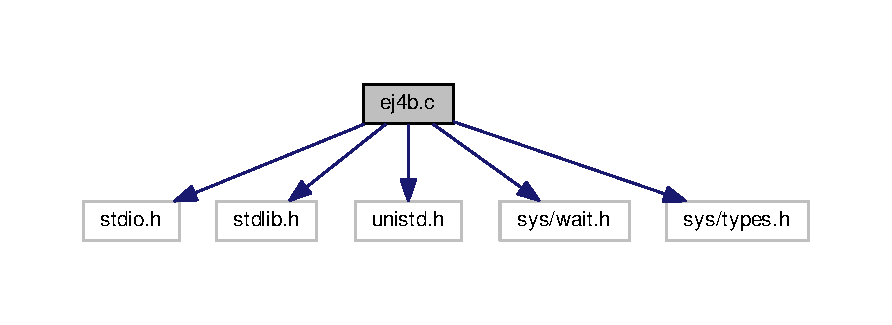
\includegraphics[width=350pt]{ej4b_8c__incl}
\end{center}
\end{figure}
\subsection*{Macros}
\begin{DoxyCompactItemize}
\item 
\hypertarget{ej4b_8c_acee2369f62e4a096d243dec3cd7d0b00}{\#define {\bfseries N\+U\+M\+\_\+\+P\+R\+O\+C}~3}\label{ej4b_8c_acee2369f62e4a096d243dec3cd7d0b00}

\end{DoxyCompactItemize}
\subsection*{Functions}
\begin{DoxyCompactItemize}
\item 
int \hyperlink{ej4b_8c_a840291bc02cba5474a4cb46a9b9566fe}{main} (void)
\begin{DoxyCompactList}\small\item\em Crea procesos Crea 8 procesos y muestras sus P\+I\+D para crear procesos huerfanos. \end{DoxyCompactList}\end{DoxyCompactItemize}


\subsection{Detailed Description}
El ejercicio 4b de la Practica 1 S\+O\+P\+E\+R. 

\begin{DoxyAuthor}{Author}
Oscar Garcia de Lara Parreño 

Santiago Gomez Aguirre 
\end{DoxyAuthor}
\begin{DoxyVersion}{Version}
1.\+0 
\end{DoxyVersion}
\begin{DoxyDate}{Date}
18-\/02-\/2016 
\end{DoxyDate}


\subsection{Function Documentation}
\hypertarget{ej4b_8c_a840291bc02cba5474a4cb46a9b9566fe}{\index{ej4b.\+c@{ej4b.\+c}!main@{main}}
\index{main@{main}!ej4b.\+c@{ej4b.\+c}}
\subsubsection[{main}]{\setlength{\rightskip}{0pt plus 5cm}int main (
\begin{DoxyParamCaption}
\item[{void}]{}
\end{DoxyParamCaption}
)}}\label{ej4b_8c_a840291bc02cba5474a4cb46a9b9566fe}


Crea procesos Crea 8 procesos y muestras sus P\+I\+D para crear procesos huerfanos. 

\begin{DoxyReturn}{Returns}
E\+X\+I\+T\+\_\+\+F\+A\+I\+L\+U\+R\+E en caso de error, E\+X\+I\+T\+\_\+\+S\+U\+C\+C\+E\+S\+S si funciona 
\end{DoxyReturn}

\hypertarget{ej5a_8c}{\section{ej5a.\+c File Reference}
\label{ej5a_8c}\index{ej5a.\+c@{ej5a.\+c}}
}


El ejercicio 5a de la Practica 1 S\+O\+P\+E\+R.  


{\ttfamily \#include $<$stdio.\+h$>$}\\*
{\ttfamily \#include $<$stdlib.\+h$>$}\\*
{\ttfamily \#include $<$sys/wait.\+h$>$}\\*
{\ttfamily \#include $<$sys/types.\+h$>$}\\*
{\ttfamily \#include $<$unistd.\+h$>$}\\*
Include dependency graph for ej5a.\+c\+:
\nopagebreak
\begin{figure}[H]
\begin{center}
\leavevmode
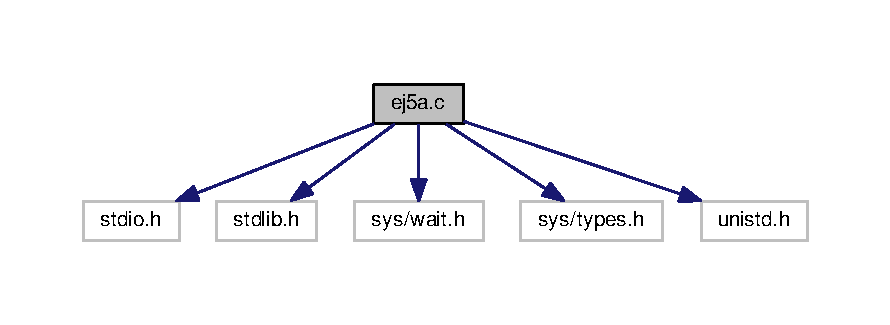
\includegraphics[width=350pt]{ej5a_8c__incl}
\end{center}
\end{figure}
\subsection*{Macros}
\begin{DoxyCompactItemize}
\item 
\hypertarget{ej5a_8c_acee2369f62e4a096d243dec3cd7d0b00}{\#define {\bfseries N\+U\+M\+\_\+\+P\+R\+O\+C}~3}\label{ej5a_8c_acee2369f62e4a096d243dec3cd7d0b00}

\end{DoxyCompactItemize}
\subsection*{Functions}
\begin{DoxyCompactItemize}
\item 
int \hyperlink{ej5a_8c_a840291bc02cba5474a4cb46a9b9566fe}{main} (void)
\begin{DoxyCompactList}\small\item\em crea hijos Crea todos los procesos de forma secuencial \end{DoxyCompactList}\end{DoxyCompactItemize}


\subsection{Detailed Description}
El ejercicio 5a de la Practica 1 S\+O\+P\+E\+R. 

\begin{DoxyAuthor}{Author}
Oscar Garcia de Lara Parreño 

Santiago Gomez Aguirre 
\end{DoxyAuthor}
\begin{DoxyVersion}{Version}
1.\+0 
\end{DoxyVersion}
\begin{DoxyDate}{Date}
18-\/02-\/2016 
\end{DoxyDate}


\subsection{Function Documentation}
\hypertarget{ej5a_8c_a840291bc02cba5474a4cb46a9b9566fe}{\index{ej5a.\+c@{ej5a.\+c}!main@{main}}
\index{main@{main}!ej5a.\+c@{ej5a.\+c}}
\subsubsection[{main}]{\setlength{\rightskip}{0pt plus 5cm}int main (
\begin{DoxyParamCaption}
\item[{void}]{}
\end{DoxyParamCaption}
)}}\label{ej5a_8c_a840291bc02cba5474a4cb46a9b9566fe}


crea hijos Crea todos los procesos de forma secuencial 

\begin{DoxyReturn}{Returns}
E\+X\+I\+T\+\_\+\+F\+A\+I\+L\+U\+R\+E en caso de error, E\+X\+I\+T\+\_\+\+S\+U\+C\+C\+E\+S\+S si funciona 
\end{DoxyReturn}

\hypertarget{ej5b_8c}{\section{ej5b.\+c File Reference}
\label{ej5b_8c}\index{ej5b.\+c@{ej5b.\+c}}
}


El ejercicio 5b de la Practica 1 S\+O\+P\+E\+R.  


{\ttfamily \#include $<$stdio.\+h$>$}\\*
{\ttfamily \#include $<$stdlib.\+h$>$}\\*
{\ttfamily \#include $<$sys/wait.\+h$>$}\\*
{\ttfamily \#include $<$sys/types.\+h$>$}\\*
{\ttfamily \#include $<$unistd.\+h$>$}\\*
Include dependency graph for ej5b.\+c\+:
\nopagebreak
\begin{figure}[H]
\begin{center}
\leavevmode
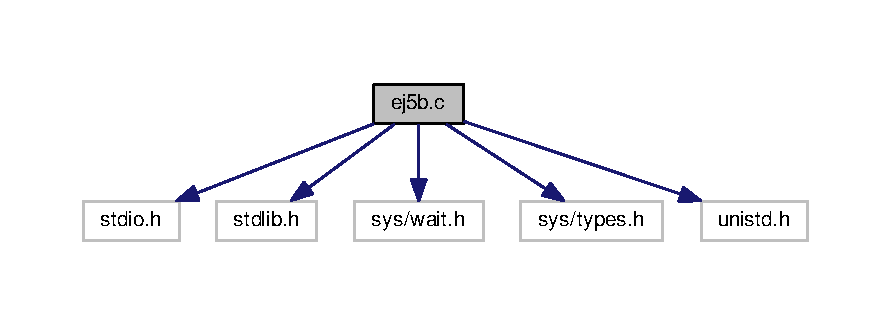
\includegraphics[width=350pt]{ej5b_8c__incl}
\end{center}
\end{figure}
\subsection*{Macros}
\begin{DoxyCompactItemize}
\item 
\hypertarget{ej5b_8c_acee2369f62e4a096d243dec3cd7d0b00}{\#define {\bfseries N\+U\+M\+\_\+\+P\+R\+O\+C}~3}\label{ej5b_8c_acee2369f62e4a096d243dec3cd7d0b00}

\end{DoxyCompactItemize}
\subsection*{Functions}
\begin{DoxyCompactItemize}
\item 
int \hyperlink{ej5b_8c_a840291bc02cba5474a4cb46a9b9566fe}{main} (void)
\begin{DoxyCompactList}\small\item\em crea hijos Crea todos los procesos y el padre espera a que terminen sus hijos \end{DoxyCompactList}\end{DoxyCompactItemize}


\subsection{Detailed Description}
El ejercicio 5b de la Practica 1 S\+O\+P\+E\+R. 

\begin{DoxyAuthor}{Author}
Oscar Garcia de Lara Parreño 

Santiago Gomez Aguirre 
\end{DoxyAuthor}
\begin{DoxyVersion}{Version}
1.\+0 
\end{DoxyVersion}
\begin{DoxyDate}{Date}
18-\/02-\/2016 
\end{DoxyDate}


\subsection{Function Documentation}
\hypertarget{ej5b_8c_a840291bc02cba5474a4cb46a9b9566fe}{\index{ej5b.\+c@{ej5b.\+c}!main@{main}}
\index{main@{main}!ej5b.\+c@{ej5b.\+c}}
\subsubsection[{main}]{\setlength{\rightskip}{0pt plus 5cm}int main (
\begin{DoxyParamCaption}
\item[{void}]{}
\end{DoxyParamCaption}
)}}\label{ej5b_8c_a840291bc02cba5474a4cb46a9b9566fe}


crea hijos Crea todos los procesos y el padre espera a que terminen sus hijos 

\begin{DoxyReturn}{Returns}
E\+X\+I\+T\+\_\+\+F\+A\+I\+L\+U\+R\+E en caso de error, E\+X\+I\+T\+\_\+\+S\+U\+C\+C\+E\+S\+S si funciona 
\end{DoxyReturn}

\hypertarget{ej8a_8c}{\section{ej8a.\+c File Reference}
\label{ej8a_8c}\index{ej8a.\+c@{ej8a.\+c}}
}


El ejercicio 8a de la Practica 1 S\+O\+P\+E\+R.  


{\ttfamily \#include $<$stdio.\+h$>$}\\*
{\ttfamily \#include $<$stdlib.\+h$>$}\\*
{\ttfamily \#include $<$unistd.\+h$>$}\\*
Include dependency graph for ej8a.\+c\+:
\nopagebreak
\begin{figure}[H]
\begin{center}
\leavevmode
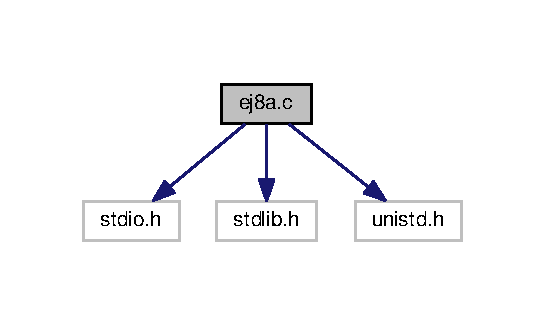
\includegraphics[width=261pt]{ej8a_8c__incl}
\end{center}
\end{figure}
\subsection*{Functions}
\begin{DoxyCompactItemize}
\item 
int \hyperlink{ej8a_8c_a3c04138a5bfe5d72780bb7e82a18e627}{main} (int argc, char $\ast$$\ast$argv)
\begin{DoxyCompactList}\small\item\em Ejecucion de comandos de la shell Ejecutamos el comando du -\/h para saber el tamaño del programa de ejecucion. \end{DoxyCompactList}\end{DoxyCompactItemize}


\subsection{Detailed Description}
El ejercicio 8a de la Practica 1 S\+O\+P\+E\+R. 

\begin{DoxyAuthor}{Author}
Oscar Garcia de Lara Parreño 

Santiago Gomez Aguirre 
\end{DoxyAuthor}
\begin{DoxyVersion}{Version}
1.\+0 
\end{DoxyVersion}
\begin{DoxyDate}{Date}
18-\/02-\/2016 
\end{DoxyDate}


\subsection{Function Documentation}
\hypertarget{ej8a_8c_a3c04138a5bfe5d72780bb7e82a18e627}{\index{ej8a.\+c@{ej8a.\+c}!main@{main}}
\index{main@{main}!ej8a.\+c@{ej8a.\+c}}
\subsubsection[{main}]{\setlength{\rightskip}{0pt plus 5cm}int main (
\begin{DoxyParamCaption}
\item[{int}]{argc, }
\item[{char $\ast$$\ast$}]{argv}
\end{DoxyParamCaption}
)}}\label{ej8a_8c_a3c04138a5bfe5d72780bb7e82a18e627}


Ejecucion de comandos de la shell Ejecutamos el comando du -\/h para saber el tamaño del programa de ejecucion. 


\begin{DoxyParams}{Parameters}
{\em argc} & numero de argumentos de entrada \\
\hline
{\em argv} & array de argumentos de entrada \\
\hline
\end{DoxyParams}
\begin{DoxyReturn}{Returns}
E\+X\+I\+T\+\_\+\+F\+A\+I\+L\+U\+R\+E en caso de error, E\+X\+I\+T\+\_\+\+S\+U\+C\+C\+E\+S\+S si funciona 
\end{DoxyReturn}

\hypertarget{ej8b_8c}{\section{ej8b.\+c File Reference}
\label{ej8b_8c}\index{ej8b.\+c@{ej8b.\+c}}
}


El ejercicio 8b de la Practica 1 S\+O\+P\+E\+R.  


{\ttfamily \#include $<$stdio.\+h$>$}\\*
{\ttfamily \#include $<$stdlib.\+h$>$}\\*
{\ttfamily \#include $<$string.\+h$>$}\\*
{\ttfamily \#include $<$sys/wait.\+h$>$}\\*
{\ttfamily \#include $<$sys/types.\+h$>$}\\*
{\ttfamily \#include $<$unistd.\+h$>$}\\*
Include dependency graph for ej8b.\+c\+:
\nopagebreak
\begin{figure}[H]
\begin{center}
\leavevmode
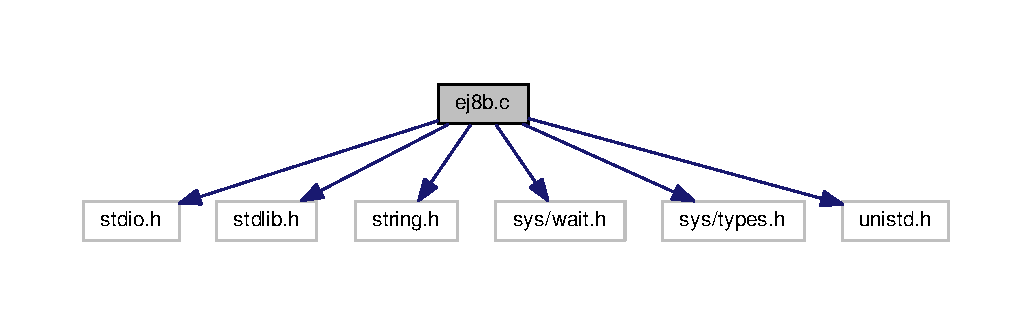
\includegraphics[width=350pt]{ej8b_8c__incl}
\end{center}
\end{figure}
\subsection*{Functions}
\begin{DoxyCompactItemize}
\item 
int \hyperlink{ej8b_8c_a3c04138a5bfe5d72780bb7e82a18e627}{main} (int argc, char $\ast$$\ast$argv)
\begin{DoxyCompactList}\small\item\em Ejecucion de comandos de la shell Ejecutamos un programa en Foreground o Background. \end{DoxyCompactList}\end{DoxyCompactItemize}


\subsection{Detailed Description}
El ejercicio 8b de la Practica 1 S\+O\+P\+E\+R. 

\begin{DoxyAuthor}{Author}
Oscar Garcia de Lara Parreño 

Santiago Gomez Aguirre 
\end{DoxyAuthor}
\begin{DoxyVersion}{Version}
1.\+0 
\end{DoxyVersion}
\begin{DoxyDate}{Date}
18-\/02-\/2016 
\end{DoxyDate}


\subsection{Function Documentation}
\hypertarget{ej8b_8c_a3c04138a5bfe5d72780bb7e82a18e627}{\index{ej8b.\+c@{ej8b.\+c}!main@{main}}
\index{main@{main}!ej8b.\+c@{ej8b.\+c}}
\subsubsection[{main}]{\setlength{\rightskip}{0pt plus 5cm}int main (
\begin{DoxyParamCaption}
\item[{int}]{argc, }
\item[{char $\ast$$\ast$}]{argv}
\end{DoxyParamCaption}
)}}\label{ej8b_8c_a3c04138a5bfe5d72780bb7e82a18e627}


Ejecucion de comandos de la shell Ejecutamos un programa en Foreground o Background. 


\begin{DoxyParams}{Parameters}
{\em argc} & numero de argumentos de entrada \\
\hline
{\em argv} & array de argumentos de entrada \\
\hline
\end{DoxyParams}
\begin{DoxyReturn}{Returns}
E\+X\+I\+T\+\_\+\+F\+A\+I\+L\+U\+R\+E en caso de error, E\+X\+I\+T\+\_\+\+S\+U\+C\+C\+E\+S\+S si funciona 
\end{DoxyReturn}

\hypertarget{ejercicio6_8c}{\section{ejercicio6.\+c File Reference}
\label{ejercicio6_8c}\index{ejercicio6.\+c@{ejercicio6.\+c}}
}


El ejercicio 6 de la Practica 3 S\+O\+P\+E\+R.  


{\ttfamily \#include $<$stdio.\+h$>$}\\*
{\ttfamily \#include $<$stdlib.\+h$>$}\\*
{\ttfamily \#include $<$string.\+h$>$}\\*
{\ttfamily \#include $<$sys/wait.\+h$>$}\\*
{\ttfamily \#include $<$sys/types.\+h$>$}\\*
{\ttfamily \#include $<$sys/ipc.\+h$>$}\\*
{\ttfamily \#include $<$errno.\+h$>$}\\*
{\ttfamily \#include $<$sys/shm.\+h$>$}\\*
{\ttfamily \#include $<$signal.\+h$>$}\\*
{\ttfamily \#include \char`\"{}semaforos.\+h\char`\"{}}\\*
Include dependency graph for ejercicio6.\+c\+:
\nopagebreak
\begin{figure}[H]
\begin{center}
\leavevmode
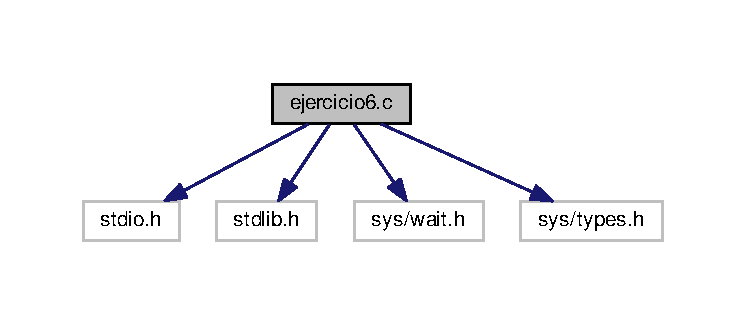
\includegraphics[width=350pt]{ejercicio6_8c__incl}
\end{center}
\end{figure}
\subsection*{Classes}
\begin{DoxyCompactItemize}
\item 
struct \hyperlink{structinfo}{info}
\begin{DoxyCompactList}\small\item\em Variables compartidas. \end{DoxyCompactList}\end{DoxyCompactItemize}
\subsection*{Macros}
\begin{DoxyCompactItemize}
\item 
\#define \hyperlink{ejercicio6_8c_a68c15c5fb7f7c6f707903e6a46ab0557}{F\+I\+L\+E\+K\+E\+Y}~\char`\"{}/bin/cat\char`\"{}
\item 
\#define \hyperlink{ejercicio6_8c_a8ae9d53f33f46cfcfcb9736e6351452a}{K\+E\+Y}~1300
\item 
\#define \hyperlink{ejercicio6_8c_a0240ac851181b84ac374872dc5434ee4}{N}~100
\end{DoxyCompactItemize}
\subsection*{Functions}
\begin{DoxyCompactItemize}
\item 
void \hyperlink{ejercicio6_8c_a52fb52fc24949b9c5e24d67f8249e0bb}{cruzando} (pid\+\_\+t pid, int dir)
\begin{DoxyCompactList}\small\item\em cruzando Imprime por pantalla cuando empieza y termina de usar el recurso \end{DoxyCompactList}\item 
void \hyperlink{ejercicio6_8c_a399eb5cae3f6bbedf44139db5c6c746a}{light\+Switch\+On} (int id\+Mutex, int id\+Recurso, \hyperlink{structinfo}{info} $\ast$buffer, int dir)
\begin{DoxyCompactList}\small\item\em light\+Switch\+On Para pedir el uso del recurso \end{DoxyCompactList}\item 
void \hyperlink{ejercicio6_8c_a69738f15e3376259e4a558cc55e49bd1}{light\+Switch\+Off} (int id\+Mutex, int id\+Recurso, \hyperlink{structinfo}{info} $\ast$buffer, int dir)
\begin{DoxyCompactList}\small\item\em light\+Switch\+Off Indicar que ya has usado el recurso \end{DoxyCompactList}\item 
\hyperlink{ejercicio6_8c_acf22f90c8a4451fe10db34ea170451b5}{coche} (int id\+Mut, int id\+Rec, \hyperlink{structinfo}{info} $\ast$buffer, int dir)
\begin{DoxyCompactList}\small\item\em coche Lo que realiza cada proceso simula que es un coche y quiere cruzar un puente(recurso) \end{DoxyCompactList}\item 
int \hyperlink{ejercicio6_8c_a0ddf1224851353fc92bfbff6f499fa97}{main} (int argc, char $\ast$argv\mbox{[}$\,$\mbox{]})
\begin{DoxyCompactList}\small\item\em Varios procesos compiten por un recurso Se creean 100 procesos, 50 se les asigna una direccion y los otros la otra, y compiten por el uso de un recurso. \end{DoxyCompactList}\end{DoxyCompactItemize}


\subsection{Detailed Description}
El ejercicio 6 de la Practica 3 S\+O\+P\+E\+R. 

\begin{DoxyAuthor}{Author}
Oscar Garcia de Lara Parreño 

Santiago Gomez Aguirre 
\end{DoxyAuthor}
\begin{DoxyVersion}{Version}
1.\+0 
\end{DoxyVersion}
\begin{DoxyDate}{Date}
28-\/03-\/2016 
\end{DoxyDate}


\subsection{Macro Definition Documentation}
\hypertarget{ejercicio6_8c_a68c15c5fb7f7c6f707903e6a46ab0557}{\index{ejercicio6.\+c@{ejercicio6.\+c}!F\+I\+L\+E\+K\+E\+Y@{F\+I\+L\+E\+K\+E\+Y}}
\index{F\+I\+L\+E\+K\+E\+Y@{F\+I\+L\+E\+K\+E\+Y}!ejercicio6.\+c@{ejercicio6.\+c}}
\subsubsection[{F\+I\+L\+E\+K\+E\+Y}]{\setlength{\rightskip}{0pt plus 5cm}\#define F\+I\+L\+E\+K\+E\+Y~\char`\"{}/bin/cat\char`\"{}}}\label{ejercicio6_8c_a68c15c5fb7f7c6f707903e6a46ab0557}
Fichero para sacar la key \hypertarget{ejercicio6_8c_a8ae9d53f33f46cfcfcb9736e6351452a}{\index{ejercicio6.\+c@{ejercicio6.\+c}!K\+E\+Y@{K\+E\+Y}}
\index{K\+E\+Y@{K\+E\+Y}!ejercicio6.\+c@{ejercicio6.\+c}}
\subsubsection[{K\+E\+Y}]{\setlength{\rightskip}{0pt plus 5cm}\#define K\+E\+Y~1300}}\label{ejercicio6_8c_a8ae9d53f33f46cfcfcb9736e6351452a}
Numero para sacar la key \hypertarget{ejercicio6_8c_a0240ac851181b84ac374872dc5434ee4}{\index{ejercicio6.\+c@{ejercicio6.\+c}!N@{N}}
\index{N@{N}!ejercicio6.\+c@{ejercicio6.\+c}}
\subsubsection[{N}]{\setlength{\rightskip}{0pt plus 5cm}\#define N~100}}\label{ejercicio6_8c_a0240ac851181b84ac374872dc5434ee4}
Numero de procesos a crear 

\subsection{Function Documentation}
\hypertarget{ejercicio6_8c_acf22f90c8a4451fe10db34ea170451b5}{\index{ejercicio6.\+c@{ejercicio6.\+c}!coche@{coche}}
\index{coche@{coche}!ejercicio6.\+c@{ejercicio6.\+c}}
\subsubsection[{coche}]{\setlength{\rightskip}{0pt plus 5cm}coche (
\begin{DoxyParamCaption}
\item[{int}]{id\+Mut, }
\item[{int}]{id\+Rec, }
\item[{{\bf info} $\ast$}]{buffer, }
\item[{int}]{dir}
\end{DoxyParamCaption}
)}}\label{ejercicio6_8c_acf22f90c8a4451fe10db34ea170451b5}


coche Lo que realiza cada proceso simula que es un coche y quiere cruzar un puente(recurso) 


\begin{DoxyParams}{Parameters}
{\em id\+Mutex} & id del semaforo mutex \\
\hline
{\em id\+Recurso} & id del semaforo del recurso \\
\hline
{\em $\ast$buffer} & direccion para acceder a las variables compartidas \\
\hline
{\em dir} & dirrecion de donde parte el proceso \\
\hline
\end{DoxyParams}
\hypertarget{ejercicio6_8c_a52fb52fc24949b9c5e24d67f8249e0bb}{\index{ejercicio6.\+c@{ejercicio6.\+c}!cruzando@{cruzando}}
\index{cruzando@{cruzando}!ejercicio6.\+c@{ejercicio6.\+c}}
\subsubsection[{cruzando}]{\setlength{\rightskip}{0pt plus 5cm}void cruzando (
\begin{DoxyParamCaption}
\item[{pid\+\_\+t}]{pid, }
\item[{int}]{dir}
\end{DoxyParamCaption}
)}}\label{ejercicio6_8c_a52fb52fc24949b9c5e24d67f8249e0bb}


cruzando Imprime por pantalla cuando empieza y termina de usar el recurso 


\begin{DoxyParams}{Parameters}
{\em pid} & pid del proceso \\
\hline
{\em dir} & dirrecion de donde parte el proceso \\
\hline
\end{DoxyParams}
\hypertarget{ejercicio6_8c_a69738f15e3376259e4a558cc55e49bd1}{\index{ejercicio6.\+c@{ejercicio6.\+c}!light\+Switch\+Off@{light\+Switch\+Off}}
\index{light\+Switch\+Off@{light\+Switch\+Off}!ejercicio6.\+c@{ejercicio6.\+c}}
\subsubsection[{light\+Switch\+Off}]{\setlength{\rightskip}{0pt plus 5cm}void light\+Switch\+Off (
\begin{DoxyParamCaption}
\item[{int}]{id\+Mutex, }
\item[{int}]{id\+Recurso, }
\item[{{\bf info} $\ast$}]{buffer, }
\item[{int}]{dir}
\end{DoxyParamCaption}
)}}\label{ejercicio6_8c_a69738f15e3376259e4a558cc55e49bd1}


light\+Switch\+Off Indicar que ya has usado el recurso 


\begin{DoxyParams}{Parameters}
{\em id\+Mutex} & id del semaforo mutex \\
\hline
{\em id\+Recurso} & id del semaforo del recurso \\
\hline
{\em $\ast$buffer} & direccion para acceder a las variables compartidas \\
\hline
{\em dir} & dirrecion de donde parte el proceso \\
\hline
\end{DoxyParams}
\hypertarget{ejercicio6_8c_a399eb5cae3f6bbedf44139db5c6c746a}{\index{ejercicio6.\+c@{ejercicio6.\+c}!light\+Switch\+On@{light\+Switch\+On}}
\index{light\+Switch\+On@{light\+Switch\+On}!ejercicio6.\+c@{ejercicio6.\+c}}
\subsubsection[{light\+Switch\+On}]{\setlength{\rightskip}{0pt plus 5cm}void light\+Switch\+On (
\begin{DoxyParamCaption}
\item[{int}]{id\+Mutex, }
\item[{int}]{id\+Recurso, }
\item[{{\bf info} $\ast$}]{buffer, }
\item[{int}]{dir}
\end{DoxyParamCaption}
)}}\label{ejercicio6_8c_a399eb5cae3f6bbedf44139db5c6c746a}


light\+Switch\+On Para pedir el uso del recurso 


\begin{DoxyParams}{Parameters}
{\em id\+Mutex} & id del semaforo mutex \\
\hline
{\em id\+Recurso} & id del semaforo del recurso \\
\hline
{\em $\ast$buffer} & direccion para acceder a las variables compartidas \\
\hline
{\em dir} & dirrecion de donde parte el proceso \\
\hline
\end{DoxyParams}
\hypertarget{ejercicio6_8c_a0ddf1224851353fc92bfbff6f499fa97}{\index{ejercicio6.\+c@{ejercicio6.\+c}!main@{main}}
\index{main@{main}!ejercicio6.\+c@{ejercicio6.\+c}}
\subsubsection[{main}]{\setlength{\rightskip}{0pt plus 5cm}int main (
\begin{DoxyParamCaption}
\item[{int}]{argc, }
\item[{char $\ast$}]{argv\mbox{[}$\,$\mbox{]}}
\end{DoxyParamCaption}
)}}\label{ejercicio6_8c_a0ddf1224851353fc92bfbff6f499fa97}


Varios procesos compiten por un recurso Se creean 100 procesos, 50 se les asigna una direccion y los otros la otra, y compiten por el uso de un recurso. 

\begin{DoxyReturn}{Returns}
E\+X\+I\+T\+\_\+\+F\+A\+I\+L\+U\+R\+E en caso de error, E\+X\+I\+T\+\_\+\+S\+U\+C\+C\+E\+S\+S si funciona 
\end{DoxyReturn}

\hypertarget{ejercicio9_8c}{\section{ejercicio9.\+c File Reference}
\label{ejercicio9_8c}\index{ejercicio9.\+c@{ejercicio9.\+c}}
}


El ejercicio 9 de la Practica 1 S\+O\+P\+E\+R.  


{\ttfamily \#include $<$stdio.\+h$>$}\\*
{\ttfamily \#include $<$stdlib.\+h$>$}\\*
{\ttfamily \#include $<$string.\+h$>$}\\*
{\ttfamily \#include $<$unistd.\+h$>$}\\*
{\ttfamily \#include $<$sys/types.\+h$>$}\\*
{\ttfamily \#include $<$sys/wait.\+h$>$}\\*
Include dependency graph for ejercicio9.\+c\+:
\nopagebreak
\begin{figure}[H]
\begin{center}
\leavevmode
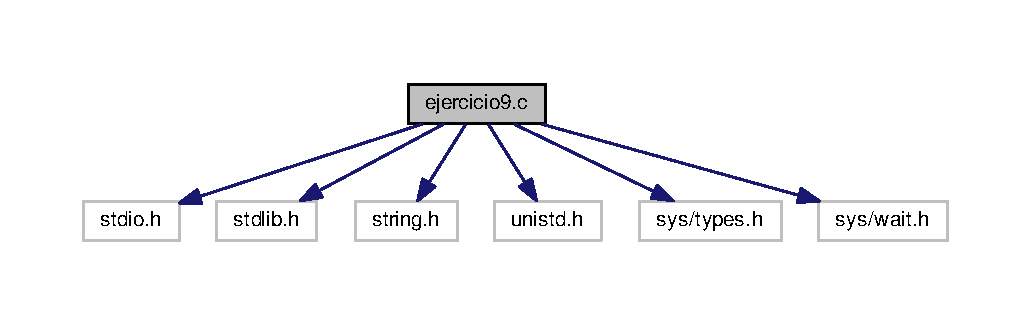
\includegraphics[width=350pt]{ejercicio9_8c__incl}
\end{center}
\end{figure}
\subsection*{Functions}
\begin{DoxyCompactItemize}
\item 
int \hyperlink{ejercicio9_8c_a840291bc02cba5474a4cb46a9b9566fe}{main} (void)
\begin{DoxyCompactList}\small\item\em tuberias Ejecutamos un programa que comunica padres e hijos a traves de tuberias, mandandose mensajes. \end{DoxyCompactList}\end{DoxyCompactItemize}


\subsection{Detailed Description}
El ejercicio 9 de la Practica 1 S\+O\+P\+E\+R. 

\begin{DoxyAuthor}{Author}
Oscar Garcia de Lara Parreño 

Santiago Gomez Aguirre 
\end{DoxyAuthor}
\begin{DoxyVersion}{Version}
1.\+0 
\end{DoxyVersion}
\begin{DoxyDate}{Date}
18-\/02-\/2016 
\end{DoxyDate}


\subsection{Function Documentation}
\hypertarget{ejercicio9_8c_a840291bc02cba5474a4cb46a9b9566fe}{\index{ejercicio9.\+c@{ejercicio9.\+c}!main@{main}}
\index{main@{main}!ejercicio9.\+c@{ejercicio9.\+c}}
\subsubsection[{main}]{\setlength{\rightskip}{0pt plus 5cm}int main (
\begin{DoxyParamCaption}
\item[{void}]{}
\end{DoxyParamCaption}
)}}\label{ejercicio9_8c_a840291bc02cba5474a4cb46a9b9566fe}


tuberias Ejecutamos un programa que comunica padres e hijos a traves de tuberias, mandandose mensajes. 

\begin{DoxyReturn}{Returns}
E\+X\+I\+T\+\_\+\+F\+A\+I\+L\+U\+R\+E en caso de error, E\+X\+I\+T\+\_\+\+S\+U\+C\+C\+E\+S\+S si funciona 
\end{DoxyReturn}

%--- End generated contents ---

% Index
\newpage
\phantomsection
\addcontentsline{toc}{chapter}{Index}
\printindex

\end{document}
